%%%%%%%%%%%%%%%%%%%%%%%%%%%%%%%%%%%%%%%%%%%%%%%%%%%%%%%%%%%%%%%%%%%%%%%%%%%%%%%%
%2345678901234567890123456789012345678901234567890123456789012345678901234567890
%        1         2         3         4         5         6         7         8

\documentclass[letterpaper, 10 pt, conference]{ieeeconf}  % Comment this line out if you need a4paper

%\documentclass[a4paper, 10pt, conference]{ieeeconf}      % Use this line for a4 paper

\IEEEoverridecommandlockouts                              % This command is only needed if 
                                                          % you want to use the \thanks command

\overrideIEEEmargins                                      % Needed to meet printer requirements.

% See the \addtolength command later in the file to balance the column lengths
% on the last page of the document

% The following packages can be found on http:\\www.ctan.org
%\usepackage{graphics} % for pdf, bitmapped graphics files
%\usepackage{epsfig} % for postscript graphics files
%\usepackage{mathptmx} % assumes new font selection scheme installed
%\usepackage{times} % assumes new font selection scheme installed
%\usepackage{amsmath} % assumes amsmath package installed
%\usepackage{amssymb}  % assumes amsmath package installed

\title{\LARGE \bf
The \textsc{TransP-0} framework for integrated transportation and power system design
}


\author{
	\IEEEauthorblockN{Dominik Ascher} \\
	\IEEEauthorblockA{
		Fakult\"at f\"ur Informatik\\
		Technische Universit\"at M\"unchen\\
		85748 Garching bei M\"unchen, Germany\\
		Email: \href{mailto:ascher@in.tum.de}{ascher@in.tum.de}
	}
	\and
	\IEEEauthorblockN{Georg Hackenberg} \\
	\IEEEauthorblockA{
		Fakult\"at f\"ur Informatik\\
		Technische Universit\"at M\"unchen\\
		85748 Garching bei M\"unchen, Germany\\
		Email: \href{mailto:hackenbe@in.tum.de}{hackenbe@in.tum.de}
	}
}


\usepackage{amsmath}
\usepackage{amssymb}
\usepackage{graphicx}
\usepackage{color}
\usepackage[colorlinks,allcolors=blue]{hyperref}
\usepackage{dblfloatfix}
\usepackage{multirow}
\usepackage{tabularx}
\usepackage{tabulary}

\newcommand{\todo}[1]{\textcolor{red}{/* #1 */}}
\newcolumntype{Y}{>{\centering\arraybackslash}X}


\begin{document}
\maketitle
\thispagestyle{empty}
\pagestyle{empty}
	\begin{abstract}
		%High penetration of electric vehicles (EV) and renewable energy sources (RES) will require fundamental changes to prevalent transportation and power systems. Intermittent and decentralized loads within the power system caused by RES and EV and the propagation of new transportation paradigms such as transportation electrification and mobility-on-demand will impose critical, closely interrelated changes on these systems.
		%Intermittent and decentralized loads caused by renewable energy sources (RES) and electric vehicles (EV) as well as 
Increasing penetration of decentralized energy production as well as the propagation of new transportation paradigms such as transportation electrification, autonomous vehicles and mobility-on-demand will require interrelated key changes to current transportation and power systems.
To diminish negative environmental impacts and achieve longterm sustainability, close integration between transportation and power systems is necessary and integrated planning, operation and control strategies have to be established. In this paper, we present TRANSP-0, a system design framework for rapid formulation and evaluation of design options within integrated transportation and power systems. Firstly, we present the TRANSP-0 design space in terms of the static parameters for integrated subsystem design. Secondly, we visit the dynamic properties of subsystem design by formulating the underlying optimal control problem. Thirdly, we establish the requirements to integrated control strategies in terms of objectives and constraints of the described optimal control problem. Finally, we conclude with an outlook on the future scope of the proposed system design framework.
	\end{abstract}
	\section{Introduction and motivation}

%Guaranteeing sustainability and minimizing negative environmental impacts are crucial challenges for transportation and power systems. Widespread adoption of electric vehicles (EVs) as well as high penetration of renewable energy sources (RES) necessitate substantial changes within these systems. 


High penetration of electric vehicles (EV) and renewable energy sources (RES) will require fundamental changes to prevalent transportation and power systems. Intermittent and decentralized loads within the power system and the propagation of new transportation paradigms such as the transportation electrification and mobility-on-demand services will impose critical, closely interrelated changes on these systems.
To guarantee sustainability and minimize negative environmental impacts, closer integration between transportation and power systems is necessary. Allan et al. ~\cite{allan2015benchmark} assess a crucial challenge for successful EV adaption in terms of their integration with supporting infrastructure systems, i.e. the transportation system, the electric power grid and supporting information systems constituting the intelligent transportation system (ITS). 
More specifically, in terms of the power system, uncontrolled charging of a high number of EVs can impose increased peak loads within the distribution network \cite{lopes2009identifying}, while increasing levels of fluctuating RES loads will impose challenges to power system operation \cite{heussen2012unified}. 
Here, the ability of plug-in electric vehicles (PEVs) to contribute to balancing the fluctuation of intermittent RES has been shown in the past \cite{dallinger2012grid}. 
%To balance EV and RES behavior, it is a major challenge for transportation systems to guarantee balanced driving behavior.
%Intermittent loads caused by RES require elaborate load balancing strategies within the power system. Increasing adoption of EV requires addressing changing mobility demands in the transportation system. 

%To comprehensively address constraints, objectives and design alternatives of both transportation and power systems, 
To comprehensively address the demands of integrated transportation and power systems, sustainable integrated planning, operation and control strategies have to be established for these systems. According strategies are frequently addressed within the concept of vehicle-to-grid (V2G), which describes a concept, where energy is released from EV batteries to the power system during times of increased power demand. By facilitating interaction between the power system and EVs, widespread V2G adaption possesses the potential to significantly reduce the amount of excess renewable energy produced within the power system and facilitates both environmental and economic benefits \cite{richardson2013electric, faria2012sustainability, mwasilu2014electric}. More specifically, key benefits of V2G include reduction of emissions, increased efficiency as well as stability and reliability of the power system \cite{yilmaz2013review}.
On the contrary, Mwasilu et al.~\cite{mwasilu2014electric} argue that for V2G adoption, central technological issues 
%such as communication delays, establishing routing protocols and cyber security 
have to be addressed first, which include rapid battery degradation of EV batteries and currently low penetration of EVs with V2G functionality.

%To handle strictly volatile energy consumers and producers such as electric vehicles and renewable energy sources, elaborate control strategies or coping mechanisms are required. 
%For instance, distribution grid operators are to decide whether grid expansion provides measurable benefits for it's voltage net users or whether increasing the percentage of smart consumers and producers provides better results.

%Given these current and future challenges and the prospected impact of RES and EVs on such systems, effective integrated control strategies to handle future power and mobility demands still have a long way to go and are subject to ongoing research. 

%Particular demands are constituted by the individual components of power and transportation systems which are subject to a diverse number of objectives and constraints. Hence, to satisfy demands within integrated transportation and power systems and guarantee sustainability elaborate multi-objective optimal control strategies for according integrated systems have to be established.

%\subsubsection*{Outline}
%
%The remainder of the article is structured as follows: Section~\ref{related_work} summarizes related work in the field as well as the contributions of this article. Section~\ref{proposed_model} describes the proposed modeling technique. Based on the proposed modeling technique and introduced model. Finally, Section~\ref{conclusion} draws a conclusion from our current state of work.
	%\section{Differentiation from related work}
%\label{related_work}
%
%In the following we first review related approaches in Section~\ref{approaches} before deriving remaining issues in Section~\ref{problems}. Then, we describe the authors' background in Section~\ref{backgrounds} before summarizing the claimed contributions in Section~\ref{contributions}.

%\subsection{Related approaches}
%\label{approaches}

Intelligent scheduling methods are widely discussed as key approaches to integrate electric vehicles into the power grid by minimizing single or multiple objectives within given power systems \cite{yang2015computational}.
% such as minimizing cost (or maximizing welfare), power losses, emissions, power deviations or optimizing battery performance of EVs within power systems \cite{yang2015computational}. 
%Here, power systems are consisted of a number of electric devices such as conventional or renewable energy sources, energy consumers as well as electric infrastructure. 
To sufficiently address technical and economic objectives for PEVs, Andreotti et al.~\cite{andreotti2012review} argue higher suitability of multi-objective optimization methods over single-objective optimization methods to evaluate model effectiveness in terms of operational limits and used objective functions. 
Zakariazadeh et al.~\cite{zakariazadeh2014multi} propose a multi-objective scheduling method for electric vehicles within a smart distribution network addressing economic and environmental objectives as well as technical constraints which manages to reduce operational costs and emissions and achieve Pareto-optimal solutions.
To achieve optimal charging decisions for EVs, Ota et al.~\cite{ota2012autonomous} propose a decentralized V2G control scheme to address the intermittency of RES energy production using electric vehicles. 
%However, the authors focus on the effects of an according charging control scheme within an isolated power system only.

%Another highly relevant direction for efficiently integrating electric vehicles into the power grid and reduce negative impacts is are approaches utilizing Vehicle Routing Problems (VRPs). Methods for vehicle routing typically focus on optimizing route selection for single or multiple traffic participants towards single or multiple objectives and a given set of constraints. Addressing objectives of energy-efficiency in terms of routing problems, Eco-Routing approaches target energy-efficient route selection. In contrast, Eco-Driving approaches target energy-efficient intermediate driving behavior ~\cite{ericsson2006optimizing}.
Felipe et al.~\cite{felipe2014heuristic} propose multiple heuristics for routing electric vehicles which consider different partial recharge strategies and recharge technologies while traveling along routes. 
Integrating both scheduling and routing approaches for EV, Barco et al.~\cite{barco2013optimal} present an approach for minimizing operation cost for battery electric vehicle (BEV) fleets, which achieves optimal routing and scheduling of charge for EV fleets.
%the approach does not consider microscopic effects on the power system when making routing and charging decisions in EVs.

%\subsection{Remaining issues}
%\label{problems}

In summary, we found that current approaches do not sufficiently address the objectives and constraints of both transportation and power systems to holistically estimate the effects of future power and transportation system scenarios. While approaches for scheduling EVs heavily address the effects of EVs within the power system, they neglect their effects on the transportation system. In contrast, routing approaches for EVs heavily address the effects of single or multiple EVs within the transportation system, in which routes are optimized, but neglect a detailed representation of the power system and it's underlying objectives.

%Here, approaches often restrict the impact of electric vehicles to decisions on charging or discharging their batteries at charging stations. However, in subsequence, individual EV objectives describing routing preferences such as shortest traveling time or energy-efficiency for EVs cannot be sufficiently taken into account. Instead, emphasis is put on the power system side, while the transportation system including traffic participants isn't represented microscopically.

%VRP
%However, approaches does not take the effects of recharging within the power system into account for general cost evaluation. 

More importantly, addressing multiple objectives when considering interfacing transportation and power systems remains a central issue for stakeholders involved when planning those systems. 
Furthermore rapid adjustment of control strategies has to be considered, when considering rapidly changing control parameters.

%Assessing the balance of the interests of transportation systems contra the power system is a challenge, which has to be tackled in the future.

%\subsection{Claimed contributions}
%\label{contributions}
%\subsection{Authors' background}
%\label{backgrounds}

In \cite{Hackenberg2012} we presented a model of the electric power system suitable for large-scale computation, which divides the power system into regions and subregions.
%, where in each time step for each region the power balance is calculated as the sum of all subregion power balances.
Then, in \cite{ascher2014early} we proposed a model which represents multi-objective traffic flows as an optimal control problem and microscopically captures the mobility demands of individual vehicles within transportation systems.
%Furthermore, the transportation infrastructure is represented as directed graph, where the edges and the distances traveled on edges represent the positions of electric vehicles.
Finally, in \cite{ascher2015integrated} we presented a systems modeling technique which allows one to microscopically model and express static and dynamic interaction between components of both power systems and transportation systems.
%which allows one to express static and dynamic interaction between components. The presented modeling approach
 %based on individual electric devices and based on individual cars in terms of components.
%We then proposed an integrated transportation and power system model, which allows to capture the respective demands of both transportation and power systems microscopically.

%\subsection{Claimed contributions}
%\label{contributions}

In this work, we describe an approach to system design for rapidly varying and evaluating parameters, objective and constraint configurations within integrated transportation and power system scenarios. 
For this, we formally describe our model for integrated transportation and power systems in terms of the microscopic behavior of individual components.
%of the transportation and power system, i.e. individual cars and electric devices.

%Substantially, in our given model, transportation and power systems are subject to a set of different demands imposed on them. 
%Within the transportation system mobility demands are expressed by passengers, who impose (1)~position preferences including origin and destination of travel as well as (2)~time preferences, which include departure and arrival times. Currently, we restrict the considered transportation modes within our model to electric vehicles.
%Within the power system, power demands are expressed by electric devices in terms of electric power loads (or energy flows) within specific times and durations. To satisfy power demands, the power system employs power generators representing different renewable energy sources.

	%\subsection{Authors' background}
\label{backgrounds}

In \cite{Hackenberg2012} we presented a model of the electric power system suitable for large-scale computation. The model divides the power system into regions and subregions. In each time step for each region the power balance is calculated as the sum of all subregion power balances.

Then, in \cite{ascher2014early} we presented a model that captures the mobility demands of individual vehicles within transportation systems. For this, the technique employs a representation which formulates multi-objective traffic flows as optimal control problems. Furthermore, the transportation infrastructure is represented as directed graph, where the edges and the distances traveled on edges represent the positions of electric vehicles.

Finally, in \cite{ascher2015integrated} we presented a component-based model which allows one to express static interaction (e.g. between vehicle and controller) as well as dynamic interaction between components (e.g. vehicle and charging station). Here, the presented modeling approach allows one to microscopically model power systems based on individual electric devices and transportation systems based on individual cars in terms of components. We then proposed an integrated transportation and power system model, which allows to capture the respective demands of both transportation and power systems microscopically.

\subsection{Claimed contributions}
\label{contributions}

In this work, we extend our previous work and formally describe our model for integrated transportation and power systems. For this, we present and detail the individual components of our model within transportation and power systems. Here, we focus on describing the microscopic behavior of individual components of the transportation and power system, i.e. individual cars and electric devices.

Substantially, in our given model, transportation and power systems are subject to a set of different demands imposed on them. Within the transportation system mobility demands are expressed by passengers, who impose (1)~position preferences including origin and destination of travel as well as (2)~time preferences, which include departure and arrival times. Currently, we restrict the considered transportation modes within our model to electric vehicles. Within the power system, power demands are expressed by electric devices in terms of electric power loads (or energy flows) within specific times and durations. To satisfy power demands, the power system employs power generators representing different renewable energy sources.

We then demonstrate our approach and employed model in a case study, where we show various scenarios for commuter traffic, which vary in terms of their traffic network structure, voltage net structure as well as employed objective weights through a number of different configurations.

	\section{The \textbf{TransP-0} design space}
%\section{The \textbf{TransP-0} integrated design abstraction}
\label{proposed_model}
The \textsc{TransP-0} design framework is intended to support both transportation and power system engineers
during early project phases 
in formulating and evaluating different design options quickly. Therefore, transportation and energy system properties - both static and dynamic - have to be captured sufficiently precise. On the other hand, the design abstraction should omit unnecessary details to enable frequent design iterations. With these requirements in mind we have developed a candidate design abstraction, which comprises various transportation and energy subsystem parameters. Note that we focused on using a minimum number of parameters, considering potentially decreased physical accuracy. However, to capture the real-world environment and establish a well-founded terminology, it is important to establish formal definitions.

%\begin{figure}[h!]
%	\begin{center}
%	\includegraphics[trim=0 10 0 0, width=0.875\columnwidth]{./gfx/system_design.png}
%	\caption{Overview over the \textsc{TransP-0} design space parameters comprising the transportation and the energy subsystem.}
%	\label{system_design}
%	\end{center}
%\end{figure}

Subsequently we formally describe the design space parameters for the transportation subsystem in Section~\ref{transport} and the energy subsystem in Section~\ref{energy_system}.

\subsection{Transportation subsystem}
\label{transport}

%why is it mesoscopic?
We decided to model the transportation subsystem in a mesoscopic fashion \cite{burghout2005mesoscopic}. In particular, our model includes a representation of the road network and the individual vehicles. The road network is modeled as a directed graph, where nodes represent intersections and edges represent road segments. Hereby, the edge weight defines the number of lanes and the edge direction indicates the intended driving direction.
%Consequently, two edges have to be used to describe bidirectional traffic flows. 
%Here, the vehicles represent ''particles'' that are traveling along the road network. 
Vehicles are assigned to points on the edges of the road network. Hence, vehicles are able to move along edges and switch between edges at intersections. The \textsc{TransP-0} abstraction of the transportation subsystem is illustrated in Figure~\ref{transport_illustration}.

\begin{figure}[h]
	\begin{center}
	\includegraphics[trim=0 6 0 21, width=.9\columnwidth]{./gfx/transportation_system.png}
	\caption{Representation of the transportation subsystem including an infrastructure (i.e.\ \textit{red} road intersections and \textit{gray} segments) and \textit{green} participants.}
	\label{transport_illustration}
	\end{center}
\end{figure}

Formally, the transportation subsystem $TS$ of the integrated design abstraction is modeled as a tuple $(TI, TP)$, where
\begin{itemize}
	\item $TI$ represents the \textit{transportation infrastructure} and
	\item $TP$ represents the \textit{traffic participants}.
\end{itemize}
Essentially, we distinguish between the static (i.e.\ the infrastructure) and the dynamic (i.e.\ the participants) parts of the transportation subsystem. In the following, we describe the the infrastructure design abstraction in Section~\ref{transport_infrastructure} before explaining the participant design abstraction in Section~\ref{participants}.

\subsubsection{Infrastructure}
\label{transport_infrastructure}

The transportation infrastructure $TI$ is modeled as a tuple $(RI, RS)$, where
\begin{itemize}
	\item $RI$ represents the \textit{road intersections} and
	\item $RS$ represents the \textit{road segments}.
\end{itemize}
Road intersections describe the nodes of the directed graph, while road segments describe the edges instead. Subsequently, we first describe road intersections in Section~\ref{intersections} before explaining road segments in Section~\ref{segments}.

\paragraph{Intersections}
\label{intersections}

The road intersections $RI$ are modeled as a tuple $(RIL, RIC)$, where
\begin{itemize}
	\item $RIL$ represents a finite set of road intersection \textit{labels} and
	\item $RIC: RIL \rightarrow \mathbb{R}^3$ represents their geometric \textit{coordinates}.
\end{itemize}
%Note that typically the coordinates are expressed in terms of latitude, longitude, and elevation (see Figure~\ref{system_design}). However, for simplicity in this work we use Cartesian coordinates instead.

\paragraph{Segments}
\label{segments}

%\textcolor{blue}{
%	Instead, the road segments $rs \in RS$ are modeled as a five-tuple $(rs_s, rs_t, rs_c, rs_e)$, where
%	\begin{itemize}
%		\item $rs_{s/t} \in RI$ represent their \textit{source} and \textit{target} road intersections,
%		\item $rs_c \in \mathbb{N}$ represents their \textit{capacities} (i.e.\ the number of lanes), and
%		\item $rs_e \in \mathbb{R}^+$ represents their \textit{efficiency} (i.e.\ a friction coefficient).
%	\end{itemize}
%	Note that the previous parameters completely determine our road segment model. Consequently, we abstract from a variety of parameters typically considered in microscopic models such as continuous elevation profiles. However, our model supports arbitrary discretization as distance between intersections and the length of edges can be chosen arbitrarily.
%}

Instead, the road segments $RS$ are modeled as a five-tuple $(RSL, RSS, RST, RSC, RSE)$, where
\begin{itemize}
	\item $RSL$ represents a finite set of road segment \textit{labels},
	\item $RSS/RST: RSL \rightarrow RIL$ represent their respective \textit{source} and \textit{target} road intersection labels and accounts for self-edges,
	\item $RSC: RSL \rightarrow \mathbb{N}$ represents their \textit{capacities} (i.e.\ the number of lanes of the road segment), and
	\item $RSE: RSL \rightarrow \mathbb{R}^+$ represents their \textit{efficiency} (i.e.\ a friction coefficient of the road segment).
\end{itemize}
Note that the previous parameters completely determine our road segment model. Consequently, we abstract from a variety of parameters typically considered in microscopic models such as continuous elevation profiles. However, our model supports arbitrary discretization as distance between intersections and the length of edges can be chosen arbitrarily.
%quelle


Furthermore, we derive the road segment distance $RSD: RSL \rightarrow \mathbb{R}_0^+$ as a mapping from road segment labels to distances using the Euclidean metric $E: \mathbb{R}^3 \times \mathbb{R}^3 \rightarrow \mathbb{R}_0^+$ such that
\[
	RSD(rsl) = E(RIC(RSS(rsl)), RIC(RST(rsl))) \textrm{.}
\]
Finally, we define road segment positions $RSP \subseteq RSL \times \mathbb{R}_0^+$ as tuples of road segment labels and traveled distances
\[
	RSP = \{(rsl, d) \in RSL \times \mathbb{R}_0^+ \mid d \leq RSD(rsl)\} \textrm{.}
\]
We use the road segment positions $RSP$ to locate traffic participants (i.e.\ vehicles) on the transportation infrastructure as explained in the following section. 
%Note that the world coordinates can be obtained by a respective coordinate transformation.

\subsubsection{Participants}
\label{participants}

The traffic participants $TP$ are modeled as a tuple $(V, D)$, where
\begin{itemize}
	\item $V$ represents the \textit{vehicles} and
	\item $D$ represents the \textit{demands}.
\end{itemize}
Consequently, we - again - distinguish between static (i.e.\ the vehicles) and dynamic (i.e.\ the demands) properties of the model. In the following, we first describe the vehicle design abstraction in Section~\ref{vehicles} before explaining the demand design abstraction in Section~\ref{demands}.

\paragraph{Vehicles}
\label{vehicles}

The vehicles $V$ are modeled as a seven-tuple $(VL, VS, VME, VP_0, VC, VEE, VSOC_0)$, where
\begin{itemize}
	\item $VL$ represents a finite set of vehicle \textit{labels},
	\item $VS: VL \rightarrow \mathbb{R}^+$ represents their \textit{size} (i.e.\ the length of the vehicle in road segment direction),
	\item $VME: VL \rightarrow \mathbb{R}^+$ represents their \textit{mechanical efficiency} (i.e. the conversion coefficient between employed energy and driven distance similar to \cite{gao2007modeling}),
	%(i.e.\ a constant ratio for conversion between electrical and mechanical energy),
	\item $VP_0: VL \rightarrow RSP$ represents their initial road segment \textit{positions} (see Section~\ref{segments}),
	\item $VC: VL \rightarrow \mathbb{R}^+$ represents their battery \textit{capacities} (i.e.\ the maximum amount of energy that can be stored by the vehicle),
	\item $VEE: VL \rightarrow \mathbb{R}^+$ represents their \textit{electrical efficiency} (i.e. the conversion coefficient between employed and stored energy),
	%(i.e.\ a constant ratio for conversion between electrical and stored energy), and
	\item $VSOC_0: VL \rightarrow \mathbb{R}^+$ represents their initial \textit{state of charge} (i.e.\ the amount of energy stored by the vehicle initially) such that
	\[
		\forall vl \in VL : VSOC_0(vl) \leq VC(vl) \textrm{.}
	\]
\end{itemize}
Note that we again abstract from many parameters which can be considered in microscopic models \cite{gao2007modeling} such as vehicle weight or exact vehicle geometry. In particular, we approximate mechanical and electrical efficiencies with constants only.

\paragraph{Demands}
\label{demands}

Finally, the demands $D$ are modeled as a four-tuple $(DL, DV, DP, DT)$, where
\begin{itemize}
	\item $DL$ represents a finite set of demand \textit{labels},
	\item $DV: DL \rightarrow VL$ represents a mapping from demand labels to \textit{vehicle} labels (i.e.\ the concerned vehicle),
	\item $DP: DL \rightarrow RSP$ represents a mapping from demand labels to road segment \textit{positions} (i.e.\ where the concerned vehicle is expected to be), and
	\item $DT: DL \rightarrow \mathbb{N}^+$ represents a mapping from demand labels to \textit{time} points (i.e.\ when the concerned vehicle is expected to be there).
\end{itemize}
Note that our abstraction is based on discrete time (see Section~\ref{dynamics}). However, we do not prescribe the time step resolution. For long travel distances and durations more coarse resolutions can be used, while for shorter distances and durations more fine-grained resolutions are typically needed.

\subsection{Power / energy subsystem}
\label{energy_system}

Similar to the transportation subsystem (see Section~\ref{transport}), we decided to model the energy subsystem in a mesoscopic fashion~\cite{Hackenberg2012}. Note that microscopic models represent the individual power lines and their physical characteristics~\cite{Dommel1968}, while macroscopic models aggregate the entire energy subsystem into a single marketplace without power line characteristics~\cite{Castronuovo2004}. Our mesoscopic model takes an intermediate approach, where only selected characteristics of the network topology are represented. In particular, we limit our representation to subnetworks of equal voltage level (i.e.\ the network \textit{regions}) and their hierarchical connectivity through transformers. Consequently, balances can be computed also for single regions rather than the entire electricity market. The \textsc{TransP-0} abstraction of the energy subsystem is illustrated in Figure~\ref{energy_illustration}.

\begin{figure}[h]
	\begin{center}
	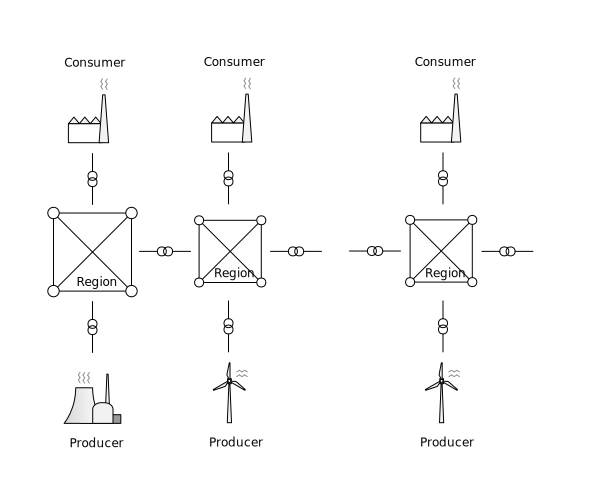
\includegraphics[trim=0 10 0 15, width=0.95\columnwidth]{./gfx/energy_system.png}
	\caption{Illustration of an energy subsystem design including an infrastructure (i.e.\ regions) and components (i.e.\ producers and consumers).}
	\label{energy_illustration}
	\end{center}
\end{figure}

Formally, the energy subsystem $ES$ of the integrated design abstraction is modeled as a tuple $(EI, EC)$, where
\begin{itemize}
	\item $EI$ represents the \textit{energy infrastructure} and
	\item $EC$ represents \textit{energy components}.
\end{itemize}
Hence, we separate network characteristics and network usage. Subsequently, we first explain the infrastructure in Section~\ref{regions} before describing the components in Section~\ref{components}.

\subsubsection{Infrastructure}
\label{energy_infrastructure}

The energy infrastructure $EI$ is modeled as a one-tuple $(R)$, where
\begin{itemize}
	\item $R$ represents the \textit{regions} of the energy infrastructure, which are determined by the voltage levels and transformers of the network.
\end{itemize}
Note that we selected a region model~\cite{Hackenberg2012} over a power flow model~\cite{Dommel1968} to reduce modeling effort and increase computational efficiency. Hence, we think it is important to enable rapid formulation and evaluation. In the following, we describe the regions in Section~\ref{regions}.

\paragraph{Regions}
\label{regions}

The network regions $R$ are modeled as a four-tuple $(RL, RC, RE, RP)$, where
\begin{itemize}
	\item $RL$ represents a finite set of region labels,
	\item $RC: RL \rightarrow \mathbb{R}^+$ represents their \textit{capacities} (i.e.\ the maximum amount of energy that can flow through each region in a predefined time interval),
	\item $RE: RL \rightarrow \mathbb{R}^+$ represents their \textit{efficiencies} (i.e.\ a constant factor determining the energy that is lost while flowing through that region), and
	\item $RP: RL \rightarrow RP \cup \{\bot\}$ represents their \textit{parent} regions (i.e.\ the superordinate voltage level or the start symbol $\bot$ for the root level).
\end{itemize}
Note that our region model represents the energy system as a tree structure. The nodes of the tree represent \textit{subnetworks} with distinct voltage levels. The edges of the tree represent \textit{transformers} connecting the subnetworks instead. The region model can be derived from existing network topologies easily.

\subsubsection{Components}
\label{components}

Instead, the energy components $EC$ are modeled as a three-tuple $(SL, ES, CS)$, where
\begin{itemize}
	\item $SL$ represents the \textit{static loads},
	\item $ES$ represents the \textit{energy storages}, and
	\item $CS$ represents the \textit{charging stations}.
\end{itemize}
In the following, we first explain the static load design abstraction in Section~\ref{static_loads}, before describing the energy storage design abstraction in Section~\ref{energy_storages} and presenting the charging station design abstraction in Section~\ref{charging_stations}. Note that currently we do not include energy producers such as generators as well as smart consumers. However, these components are subject for our future work.

\paragraph{Static loads}
\label{static_loads}

The static loads $SL$ are modeled as a three-tuple $(SLL, SLP, SLR)$, where
\begin{itemize}
	\item $SLL$ represents a finite set of static load \textit{labels},
	\item $SLP: SLL \rightarrow (\mathbb{N} \rightarrow \mathbb{R})$ represents a mapping from static load labels $SLL$ to static load \textit{profiles} (i.e.\ a predefined production and consumption curve), and
	\item $SLR: SLL \rightarrow RL$ represents a mapping from static load labels to parent \textit{regions} (i.e.\ the region where the static load is attached).
\end{itemize}
Note that static load profiles associate a numeric load to each discrete time step. Hereby positive loads represent energy production and negative loads represent energy consumption. Consequently, static loads can be used to model everything from home appliances over solar panels to conventional power generators. In particular, we assume such loads to be uncontrollable from the perspective of the engineers.

\paragraph{Energy storages}
\label{energy_storages}

Then, the energy storages $ES$ are modeled as a five-tuple $(ESL, ESCA, ESE, ESS_0, ESR)$, where
\begin{itemize}
	\item $ESL$ represent a finite set of energy storage \textit{labels},
	\item $ESC: ESL \rightarrow \mathbb{R}^+$ represents their \textit{capacities} (i.e.\ the maximum amount of energy that can be stored),
	\item $ESE: ESL \rightarrow \mathbb{R}^+$ represents their energy storage \textit{efficiencies} (i.e. the conversion coefficient between  and stored energy), and
	\item $ESS_0: ESL \rightarrow \mathbb{R}_0^+$ represents their initial \textit{state of charges} (i.e.\ the amount of energy stored initially) such that
	\[
		ESS_0(esl) \leq ESC(esl) \textrm{, and}
	\]
	\item $ESR: ESL \rightarrow RL$ represents their parent \textit{regions} (i.e.\ the region where the energy storage is attached).
\end{itemize}
Note that the energy storage model is analogous to the electric vehicle model described in Section~\ref{vehicles}. However, electric vehicles additionally define mechanical parameters, while energy storages are attached to regions statically. Furthermore, we currently target small batteries rather than large storage facilities. Note that the latter might require additional parameters. 
%Larger facilities require additional parameters~\cite{?}.

\paragraph{Charging stations}
\label{charging_stations}

Finally, the charging stations $CS$ are modeled as a four-tuple $(CSL, CSP, CSE, CSR)$, where
\begin{itemize}
	\item $CSL$ represents a finite set of charging station \textit{labels},
	\item $CSE: CSL \rightarrow \mathbb{R}^+$ represents their \textit{efficiencies} (i.e.\ a constant loss factor for respective energy flows), and
	\item $CSP: CSL \rightarrow RSL$ represents their \textit{positions}, i.e.\ road segment labels with zero road segment distance
	\[
		RSD(CSP(csl)) = 0 \textrm{, and}
	\]
	\item $CSR: CSL \rightarrow RL$ represents their parent \textit{regions} (i.e.\ the region where the charging station is attached).
\end{itemize}
Note that the charging station position mapping $CSP$  and the charging station region mapping $CSR$ define the static connections between the transportation subsystem and the energy subsystem. Consequently, vehicles (see Section~\ref{vehicles}) are able to interact with arbitrary regions (see Section~\ref{regions}) of the energy subsystem infrastructure at predefined zero-length road segments (see Section~\ref{segments}).

	\section{Discrete-time \textbf{TransP-0} dynamics}
\label{dynamics}

While the previous section was only concerned with the static parameters, i.e. the design space of integrated transportation and energy system design, this section focuses on dynamic aspects instead. In effect, each system design defines an optimal control problem (or dynamic programming problem)~\cite{Bertsekas1995} over the transportation and energy subsystem dynamics. We decided to use a discrete-time model of the system dynamics due to the high problem dimensionality involved in its control. In the following, we describe the respective state space in Section~\ref{states}, the action space in Section~\ref{actions}, and the transition function in Section~\ref{transitions}. Note that the states, actions, and transition function do not have to be defined by the transportation and power system engineers. Rather, the definitions are equal for all system designs expressed with the \textsc{TransP-0} abstraction.

\subsection{States}
\label{states}

The overall system states $S_t \in \mathbb{S}$ with time point $t \in \mathbb{N}$ of the optimal control problem are modeled as a four-tuple $(VS_t, ESS_t, CSS_t, RS_t)$, where
\begin{itemize}
	\item $VS_t$ represents the \textit{vehicle states},
	\item $ESS_t$ represents the \textit{energy storage states},
	\item $CSS_t$ represents the \textit{charging station states}, and
	\item $RS_t$ represents the \textit{region states}.
\end{itemize}
Note that we do not associate a state with the infrastructure of the transportation subsystem (i.e.\ we assume the infrastructure to be constant). In the following, we describe the vehicle states in Section~\ref{states_vehicles}, the energy storage states in Section~\ref{states_storages}, the charging station station states in Section~\ref{states_stations}, and the region states in Section~\ref{states_regions}.

\subsubsection{Vehicle states}
\label{states_vehicles}

The vehicle states $VS_t$ are modeled as a tuple $(VP_t, VSOC_t)$, where
\begin{itemize}
	\item $VP_t: VL \rightarrow RSP$ represents their current road segment \textit{positions} and
	\item $VSOC_t: VL \rightarrow \mathbb{R}_0^+$ represents their current \textit{state of charge}.
\end{itemize}
Consequently, our design abstraction neglects effects such as changing vehicle weights due to passenger load or changing tire and road friction coefficients~\cite{imine2006road}.
%due to wheel temperatures
Instead, we omitted such effects to ease design formulation~\cite{gao2007modeling} and employed mechanical efficiency coefficients $VME$ (see Section~\ref{vehicles}), which have to be selected carefully to achieve desired effects.

\subsubsection{Energy storage states}
\label{states_storages}

In contrast, the energy storage states $ESS_t$ are modeled as a one-tuple $(ESOC_t)$, where
\begin{itemize}
	\item $ESOC_t: ESL \rightarrow \mathbb{R}_0^+$ represents their current \textit{state of charge}. 
\end{itemize}
Note that we omitted advanced effects such as wear of equipment, 
%~\cite{chawla2010utility}
which can cause degrading storage efficiency. Again, we believe that such effects can be neglected during early phase system-level design. Furthermore, depending on the time step resolution additional state parameters are required to model - for example - ramp-up times of pumped storage hydro power plants~\cite{Garcia2008}.

\subsubsection{Charging station states}
\label{states_stations}

Then, the charging stations states $CSS_t$ are modeled as a one-tuple $(CSB_t)$, where
\begin{itemize}
	\item $CSB_t: CSL \rightarrow \mathbb{R}$ represents their current \textit{balance} (i.e.\ the energy transferred from or to a connected vehicle).
\end{itemize}
In an advanced version of the design abstraction one could also consider failure states or software control states of charging stations. For now we assume that all charging stations work properly. Furthermore, the control strategy is provided implicitly by the optimal control problem formulation.

\subsubsection{Region states}
\label{states_regions}

Finally, the region states $R_t$ are modeled as a three-tuple $(RE_t^<, RE_t^>, RB_t)$, where
\begin{itemize}
	\item $RE_t^\sim: RL \rightarrow \mathbb{R}, \sim \in \{<,>\}$ represents their current aggregate \textit{energy} production (i.e.\ $\sim = >$) and consumption (i.e.\ $\sim = <$) values (obtained from the subregions and subcomponents) and
	\item $RB_t: RL \rightarrow \mathbb{R}$ represents their current \textit{balances} (i.e.\ the aggregated loads).
\end{itemize}
Again, we neglect physical state parameters such as power line temperatures or failure modes (e.g.\ due to exceeded temperature limits or due to environmental influences). Consequently, we assume that the energy subsystem infrastructure is available during entire system operation. In an advanced version of the design abstraction one might also consider failure modes and respective repair actions~\cite{anghel2007stochastic} as well as additional topological and physical characteristics.

\subsection{Actions}
\label{actions}

The actions $A_t \in \mathbb{A}$ with time point $t \in \mathbb{N}$ of the optimal control problem are modeled as a tuple $(VA_t, ESA_t)$, where
\begin{itemize}
	\item $VA_t$ represents the \textit{vehicle actions} and
	\item $ESA_t$ represents the \textit{energy storage actions}.
\end{itemize}
Note that vehicles and energy storages are the only system components comprising actions. The states of the other components is influenced directly or indirectly by these actions. In the following, we describe the vehicle actions in Section~\ref{actions_vehicles} before explaining the energy storage actions in Section~\ref{actions_storages}.

\subsubsection{Vehicle actions}
\label{actions_vehicles}

The vehicle actions $VA_t$ are modeled as a three-tuple $(VR_t, VS_t, VB_t)$, where
\begin{itemize}
	\item $VR_t: VL \rightarrow (\mathbb{N} \rightarrow RSL)$ represents their respective \textit{route}, i.e.\ a sequence of connected road segments with $\forall vl \in VL, n \in \mathbb{N}:$
	\[
		RST(VR_t(vl)(n)) = RSS(VR_t(vl)(n + 1))
	\]
	starting at the previous vehicle road segment position with $\forall vl \in VL$ and $VP_{t-1}(vl) = (rsl, d):$
	\[
		VR_t(vl)(0) = rsl \textrm{,}
	\]
	\item $VS_t: VL \rightarrow \mathbb{R}_0^+$ represents their current \textit{speed}, and
	\item $VB_t: VL \rightarrow \mathbb{R}$ represents their current \textit{balances} (i.e.\ the amount of energy sent to or received from a charging station) such that
	\[
		\forall vl \in VL: VB_t(vl) \neq 0 \textrm{ only if }
	\]
	the current vehicle speed is zero, i.e.\
	\[
		 VS_t(vl) = 0 \textrm{ and }
	\]
	the vehicle is located currently at a charging station, i.e.\
	\[
		\exists csl \in CSL: VP_t(vl) = (CSP(csl), 0) \textrm{.}
	\]
\end{itemize}
Note that the routes $VR_t$ have to cover the distances traveled by each vehicle with the respective vehicle speeds $VS_t$ in each time step. Hereby, the vehicle speed also can be zero such that the route only contains the current road segment. In particular, zero speed is required to park vehicles at charging stations for one time step. Consequently, the time step resolution also determines the time intervals for charging or discharging vehicle batteries. Furthermore, note that we neglect accelerations and decelerations in the model, which might have a considerable effect on energy consumption~\cite{gao2007modeling}. Instead, we assume ideal conditions, which we believe to be sufficient for early phase system design evaluation.

\subsubsection{Energy storage actions}
\label{actions_storages}

The energy storage actions $ESA_t$ are modeled as a one-tuple $(ESB_t)$, where
\begin{itemize}
	\item $ESB_t: ESL \rightarrow \mathbb{R}$ represents their current \textit{balances} (i.e.\ the amount of energy sent to or received from the parent region).
\end{itemize}
Note that physically one cannot control the (positive or negative) energy balance directly. Rather, for a pumped storage hydro power plant one might control a valve limiting the downhill water flow and an electric drive causing the uphill water flow~\cite{Castronuovo2004}. In fact, the actual control parameters depend on the concrete storage type. We believe that considering the energy balance directly represents the smallest common denominator and, hence, most suitable abstraction in terms of its coverage.

\subsection{Transition function}
\label{transitions}

Finally, the transition function $T$ of the optimal control problem is modeled as a deterministic mapping $\mathbb{S} \times \mathbb{A} \rightarrow \mathbb{S}$ with transitions $T(S_t, A_t) = S_{t+1}$ and time point $t \in \mathbb{N}$, where
\begin{itemize}
	\item $S_t$ represent the system \textit{state} at time point $t$,
	\item $A_t$ represents the \textit{action} applied to state $S_t$, and
	\item $S_{t+1}$ represents the system \textit{state} at time point $t+1$.
\end{itemize}
Note that we work with a deterministic transition function to reduce the complexity of the system dynamics. Consequently, one can solve the optimal control problem more easily in practice~\cite{Bertsekas1995}. However, to obtain higher physical accuracy one might need to introduce a non-deterministic or even probabilistic transition function instead. This transition function could encode the uncertainty about the physical process involved, which occurs due to various simplifications made (see Sections~\ref{proposed_model} and~\ref{dynamics}).

Having in mind that $S_t = (VS_t, ESS_t, CSS_t, RS_t)$ and $A_t = (VA_t, ESA_t)$ we decompose $T$ into partial transition functions $VTF,ESTF,CSTF,RTF$, where
\begin{itemize}
	\item $VS_{t+1} = VTF(VS_t, VA_t)$ represents the \textit{vehicle transition function},
	\item $ESS_{t+1} = ESTF(ESS_t, ESA_t)$ represents the \textit{energy storage transition function},
	\item $CSS_{t+1} = CSTF(VS_{t+1}, VA_t)$ represents the \textit{charging station transition function}, and
	\item $RS_{t+1} = RTF(CSS_{t+1}, ESS_{t+1})$ represents the \textit{region transition function}.
\end{itemize}
Subsequently, we describe the transitions functions for vehicles in Section~\ref{transitions_vehicles}, for energy storages in Section~\ref{transitions_storages}, for charging stations in Section~\ref{transitions_stations}, and for regions in Section~\ref{transitions_regions}.  
%vehicle transition function in Section~\ref{transitions_vehicles}, the energy storage transition function in Section~\ref{transitions_storages}, the charging station transition function in Section~\ref{transitions_stations}, and the region transition function in Section~\ref{transitions_regions}.

\subsubsection{Vehicle transition function}
\label{transitions_vehicles}

We decompose the vehicle transition function $VTF$ into two partial transition functions $VPTF,VSOCTF$, where
\begin{itemize}
	\item $VP_{t+1} = VPTF(VP_t, VR_t, VS_t)$ represents the \textit{vehicle position transition function} mapping the current position, route, and speed to the next position and
	\item $VSOC_{t+1} = VSOCTF(VSOC_t, VP_t, VR_t, VS_t, VB_t)$ represents the \textit{vehicle state of charge transition function} mapping the current state of charge, position, route, speed, and balance to the next state of charge.
\end{itemize}
Note that the position transition function requires the road segment distances $RSD$ (see Section~\ref{vehicles}) to compute the follow-up vehicle positions on their routes. Furthermore, the vehicle state of charge transition function either requires the driving information (i.e.\ the position, route, and speed) or the charging balance information (i.e.\ the energy flow through the charging station) to compute the follow-up state of charge. For future work, we plan on integrating neural networks for energy consumption estimation to achieve increased estimation accuracy \cite{felipe2015energy}.

\subsubsection{Energy storage transition function}
\label{transitions_storages}

In contrast, we decompose the energy storage transition function $ESTF$ into one partial transition function $ESSTF$, where
\begin{itemize}
%	\item $ESS_{t+1} = ESSTF(ESS_t, ESB_t)$ represents the \textit{energy storage state of charge transition function} mapping the current state of charge and balance to the next state of charge such that $\forall esl \in ESL$ with $ESB_t(esl) < 0:$
%	\[
%		ESS_{t+1}(esl) = 
%		\begin{cases}
%		ESS_t(esl) - (1+ESE(esl)) * ESB_t(esl) & \enspace \textrm{if } ESB_t \geq 0 \\
%		ESS_t(esl) - (1-ESE(esl)) * ESB_t(esl) & \enspace \textrm{otherwise}
%		\end{cases}
%		\textrm{, and}
%	\]
	\item $ESS_{t+1} = ESSTF(ESS_t, ESB_t)$ represents the \textit{energy storage state of charge transition function} mapping the current state of charge and balance to the next state of charge such that $\forall esl \in ESL$ with $ESB_t(esl) < 0:$
	\[
	 ESS_{t+1}(esl) = ESS_t(esl) - (1+ESE(esl)) * ESB_t(esl)
	\]
	and for $\forall esl \in ESL$ with $ESB_t(esl) \geq 0:$
	\[
	ESS_{t+1}(esl) = ESS_t(esl) - (1-ESE(esl)) * ESB_t(esl)
	\]
	
\end{itemize}
Note that we use the energy storage efficiency $ESE$ (see Section~\ref{energy_storages}) to compute the state of charge during charging. Hereby, the efficiency factor models the energy loss during energy conversion (e.g.\ electric to potential energy). 
%In particular, the factor models the combined loss in both directions. Therefore, during discharging the factor is not used.

\subsubsection{Charging station transition function}
\label{transitions_stations}

Then, we decompose the charging station transition function $CSTF$ into one partial transition function $CSBTF$, where
\begin{itemize}
	\item $CSB_{t+1} = CSBTF(VP_{t+1}, VB_t)$ represents the \textit{charging station balance transition function} mapping the vehicle road segment positions and balances to the charging station balances such that $\forall csl \in CSL$ with $\exists vl \in VL: VP_{t+1}(vl) = (csl, 0):$
	\[
		CSB_{t+1}(csl) = VB_{t}(vl) \textrm{.}
	\]
\end{itemize}
Consequently, the charging station balance equals the vehicle balance.

\subsubsection{Region transition function}
\label{transitions_regions}

Finally, we decompose the region transition function $RTF$ into three partial transition functions $RETF^<,RETF^>,RBTF$, where
\begin{itemize}
	\item $RE_{t+1}^\sim = RETF^\sim(ESB_{t+1}, CSB_{t+1})$ with $\sim \in \{<,>\}$ represent the \textit{region energy transition functions} aggregating the associated static load profiles, energy storage balances, charging station balances, and subregion balances such that $\forall rl \in RL:$
		\begin{equation*}
		\begin{split}
		RE_{t+1}^\sim = & \sum_{sll \in SLL: SLR(sll) = rl} F_\sim(SLP(sll)(t+1)) + \\
		& \sum_{esl \in ESL: ESR(esl) = rl} F_\sim(ESB_{t+1}(esl)) + \\
		& \sum_{csl \in CSL: CSR(csl) = rl} F_\sim(CSB_{t+1}(csl)) + \\
		& \sum_{rl' \in RL: RP(rl') = rl} F_\sim(RB_{t+1}(rl')) \textrm{, where} \\
		\end{split}
		\end{equation*}
	the function $F_\sim: \mathbb{R} \rightarrow \mathbb{R}$ with $\sim \in \{<,>\}$ filters the production and consumption values such that
	\[
		F_\sim(x) = \begin{cases}
			x & \quad \textrm{if } x \sim 0 \\
			0 & \quad \textrm{otherwise}
		\end{cases}
		\textrm{, and}
	\]
	\item $RB_{t+1} = RBTF(ESB_{t+1}, CSB_{t+1})$ represents the \textit{region balance transition function} calculating the final balance from the aggregate production and consumption values such that $\forall rl \in RL:$
	\[
		RB_{t+1}(rl) = RE_{t+1}^< * (1 + RE(rl)) +
	\]
	\[
		RE_{t+1}^> * (1 - RE(rl)) \textrm{.}
	\]
	where the balance indicator is then
	\[
		RB_{t+1} = \begin{cases}
		RB_{t+1} * (1 + RE(rl)) & \textrm{if } RB_{t+1} \sim 0 \\
		RB_{t+1} & \textrm{otherwise}
		\end{cases}
	\]
	
	\[
		RB_P =	RE_{t+1}^> * (1 + RE(rl)) + RE_{t+1}^< 
	\]	
	\[
		RB_C =	RE_{t+1}^< * (1 - RE(rl)) + RE_{t+1}^> 
	\]	
\end{itemize}
Note that the partial transition functions are defined recursively. Consequently, first the productions, consumptions, and balances have to be computed for the lowest-level regions (i.e.\ the regions without subregions). Then, the upper levels can be derived one after the other. Furthermore, note that the balance transition function multiplies the production and consumption values with the region efficiency factor $RE$. In particular, the consumption is increased and the production is decreased by the factor to account for losses over the power lines. Hereby, the efficiency $RE$ typically ranges in the area of a few percent only and the factor is lower for higher voltage levels.
	
\section{Objectives and Constraints}
\subsection{Constraints}
\label{constraints}

In principle, one can define arbitrary constraints over the static and dynamic system properties presented in the previous sections. In particular, we believe that such constraints might arise from design decisions made by transportation and energy system engineers. Hence, we do not want to prescribe the constraints. Rather, we provide two basic constraints which we believe to be part of any integrated system design. The first constraint makes sure that the road segment capacities $RSC$ (i.e.\ the number of lanes) of the transportation subsystem infrastructure $TSI$ are not exceeded (see Section~\ref{collisions}). The second constraint makes sure that the region capacities $RC$ of the energy subsystem infrastructure $ESI$ are not exceeded (see Section~\ref{capacities}).

\subsubsection{Segment capacities}
\label{collisions}

TODO

%Overlapping vehicle pairs $OVP : \mathbb{VS} \rightarrow V \times V$
%\[
%OVP(VS) = \{(v_1, v_2) \in V \times V \mid
%\]
%\[
%((rs_1,rd_1),\cdot) \in VS(v_1), ((rs_2,rd_2),\cdot) \in VS(v_2) :
%\]
%\[
%rs_1 = rs_2 \wedge (|rd_1 - rd_2| < VL(v_1) / 2
%\]
%\[
%\vee
%\]
%\[
%|rd_1 - rd_2| < VL(v_2) / 2)\}
%\]
%Overlapping vehicle sets $OVS : \mathbb{VS} \times V \rightarrow \mathcal{P}(V)$
%\[
%OVS(VS,v) = \{v' \in V \mid (v, v') \in OVP(VS)\}
%\]
%Collision property $CV : \mathbb{VS} \rightarrow \mathbb{B}$
%\[
%CV(VS) \Leftrightarrow \exists v \in V :
%\]
%\[
%|OVS(VS, v)| > RSL(rs) \text{ with } ((rs,\cdot),\cdot) = VS(v)
%\]

\subsubsection{Region capacities}
\label{capacities}

TODO

\subsection{Objectives}
\label{objectives}

In addition to constraints (see Section~\ref{constraints}), our approach supports arbitrary objectives over the static and dynamic properties of the transportation system (see Section~\ref{transport}) and the energy system (see Section~\ref{energy_system}). In particular, we do not want to prescribe any particular objectives. Rather, we believe that it is the designers task to formulate different objectives and explore their effect on the system structure and dynamics. For demonstration (see Section~\ref{demonstration}) we selected objective that we have used also in previous work. Among these objective we consider minimizing traveling times, minimizing energy consumption during driving, and minimizing the energy disbalance of the energy subsystem. Other objectives might include for example minimizing the free road segment space or minimizing the energy storage usage.
	%\section{Using the \textbf{TransP-0} design abstraction}
\label{demonstration}

In the following, we evaluate \textsc{TransP-0}. Therefore, we first present prototypical tool support in Section~\ref{tool}, which we have used for coding the actual system designs and optimizing their behavior. Then, we describe the sample system design in Section~\ref{examples}, which are intended to show the capabilities of the design abstraction. Finally, we discuss the results of and experiences made during the experiments in Section~\ref{discussion}. In particular, we are interested in the suitability of the design abstraction with respect to rapid and iterative design formulation as well as evaluation.

\subsection{Prototypical tool support}
\label{tool}

TODO

\begin{figure}[h]
	\includegraphics[width=\columnwidth]{./gfx/modeling.png}
	\caption{System modeling using regular Java classes and the Eclipse integrated development environment (IDE).}
	\label{figure:modeling}
\end{figure}

TODO

\begin{figure}[h]
	\includegraphics[width=\columnwidth]{./gfx/analysis.png}
	\caption{Model analysis using a basic approximate dynamic programming algorithm and comprehensive visualization techniques.}
	\label{figure:analysis}
\end{figure}

TODO

\subsection{Exemplary system designs}
\label{examples}

To demonstrate the proposed approach and underlying model, we propose several scenarios for commuter traffic. In each scenario, in order to reach their location of work, ten traffic participants travel between home to work locations. Travel is subject to specified time windows, which are imposed on arrival and leaving times at the specific locations, i.e. home and work. The demonstration then evaluates the behavior of typical work commute on transportation and power systems within small scale scenarios, which vary the structure of the underlying infrastructure as well as the employed objectives and constraints.

Subsequently, we evaluate our systematic approach using different traffic scenarios with different configurations varying in their respective parameters and structure of cost functions. Note that at this point we do not consider varying constraints. 


%Hence, in each time step traffic participants actions consist in selecting driving speed, time of charging, time of departure as well as route selection when driving towards their respective destination positions. 

For all scenarios in general, we employ a traffic infrastructure which is consisted of a traffic network of 20 by 5 kilometers with two possible origins and two possible destinations of travel for individual traffic participants. At its most basic level, the traffic infrastructure is consisted of a basic structure, where two origin-destination pairs are connected. We then introduce an extended traffic infrastructure, which features additional pathways, which can possibly allow for more energy-efficient or less congested routes between respective origin and destinations.

Furthermore, we employ a electric network structure, featuring a single voltage net for all consumers and producers. Then, we introduce another structure of the electric network, which distinguishes two voltage nets for each home and work consumers and producers.

\begin{figure}
	\centering
	\includegraphics[width=\columnwidth]{gfx/profiles.PNG}
	\caption{Illustration of home (H0) and workplace (G0) load profiles.}
	\label{profiles}
\end{figure}

We vary scenario configuration with regard to the objective function, voltage net and traffic network structure. Subsequently we describe the according measures of variation.

\subsubsection{Objective function structure}

The objective function structure concerns the weighting and structure of individually employed objective functions. In the presented example scenarios, we vary cost functions with regard to vehicle energy-efficiency and vehicle shortest-traveling time objectives and the respective weighting of these cost functions. 

\subsubsection{Voltage net structure}
Voltage net structure is expressed by the underlying tree-like overall electric net infrastructure. More specifically, it concerns the number of employed low voltage nets for a given model excerpt. In the presented example scenarios, we alternate between assigning one or multiple distinct voltage nets to a group of consumers or producers based on their locality.

\subsubsection{Traffic network structure}
Traffic network structure concerns the number of available intersections as well as their connected segments making up the traffic infrastructure. In general, the traffic infrastructure can be changed by adding additional interactions or segments, allowing for a wider variety of resulting routes to be chosen by the traffic participants, e.g. enabling more energy-efficient or shorter routes.

\subsubsection{Results}
The results are pictured in Figure \ref{figure:examples}. 

\begin{table*}[b]
	\centering
	\renewcommand{\arraystretch}{1.3}
	\begin{tabularx}{\textwidth}{|Y|Y|Y|Y|}
		\hline
		
		\textbf{Scenario 1} & \textbf{Scenario 2} & \textbf{Scenario 3} \\
		
		\hline
		
		Energy-efficiency &
		Shortest traveling time &
		Intermediate \\
		
		\hline
		
		\includegraphics[width=0.20\textwidth, trim=0 0 0 -3]{gfx/Graph2.png} &
		\includegraphics[width=0.20\textwidth, trim=0 0 0 -3]{gfx/Graph1.png} &
		\includegraphics[width=0.20\textwidth, trim=0 0 0 -3]{gfx/Graph1.png} \\
		
		\hline
		
		\includegraphics[width=0.20\textwidth, trim=0 0 0 -3]{gfx/Graph2.png} &
		\includegraphics[width=0.20\textwidth, trim=0 0 0 -3]{gfx/Graph1.png} &
		\includegraphics[width=0.20\textwidth, trim=0 0 0 -3]{gfx/Graph1.png} \\
		\hline			
	\end{tabularx}
	\caption{Traffic flow graph and power charts for different configurations.}
	\label{figure:examples}
\end{table*}
	%\subsection{Design abstraction evaluation}
\label{discussion}

Demonstration results obtained with the conducted case study show the feasibility of our approach to adapt to changing scenario configurations and varying scenario parameters. In previous work \cite{ascher2015integrated} we evaluated our approach with regard to it's validity, novelty, efficiency and applicability. 

The case study employs static profiles based on distribution operator load profiles for home and workplace locations. We demonstrated a set of future scenarios, where electric vehicles are prevalent and are employed heavily within the transportation system.

	\section{Conclusion}
\label{conclusion}

%\todo{Write conclusion. How far are we in modeling the problem? When can we use the model for real-world scenarios? How far are we in solving the problem?}

%\todo{Effect of EVS on individual systems, stabilization of power system demands}.

Charging and discharging electric vehicles (EV) as well as high penetration of renewable energy sources (RES) will prove tough challenges for power and transportation systems in the future. In this paper, we presented an approach for establishing optimal control strategies to deal with potentially challenging future scenarios. We presented formal formulations for our model in terms of the individual components of transportation and power systems. We demonstrated the feasibility of our approach with a set of incremental scenarios. However, while our approach offers advantages with regard to it's comprehensive planning strategies, the validity of our approach has to be evaluated in the future. Future work includes establishing large-scale integrated planning strategies and assessing their applicability for multi-modal passenger transportation and logistics problems.

	
	\bibliographystyle{bst/IEEEtran}
	\bibliography{references}




\end{document}
